\documentclass{article}

\usepackage{graphicx}
\usepackage{tikz}
\usepackage{tikzsymbols}
\usetikzlibrary{calc,patterns,shapes.geometric}
\pagestyle{empty}
\usepackage[margin=0pt]{geometry}
\geometry{papersize={14in,12in}}

\def\centerarc[#1](#2)(#3:#4:#5){\draw[#1] ($(#2)+({#5*cos(#3)},{#5*sin(#3)})$) arc (#3:#4:#5);}

\begin{document}
	\begin{figure}
		\centering
		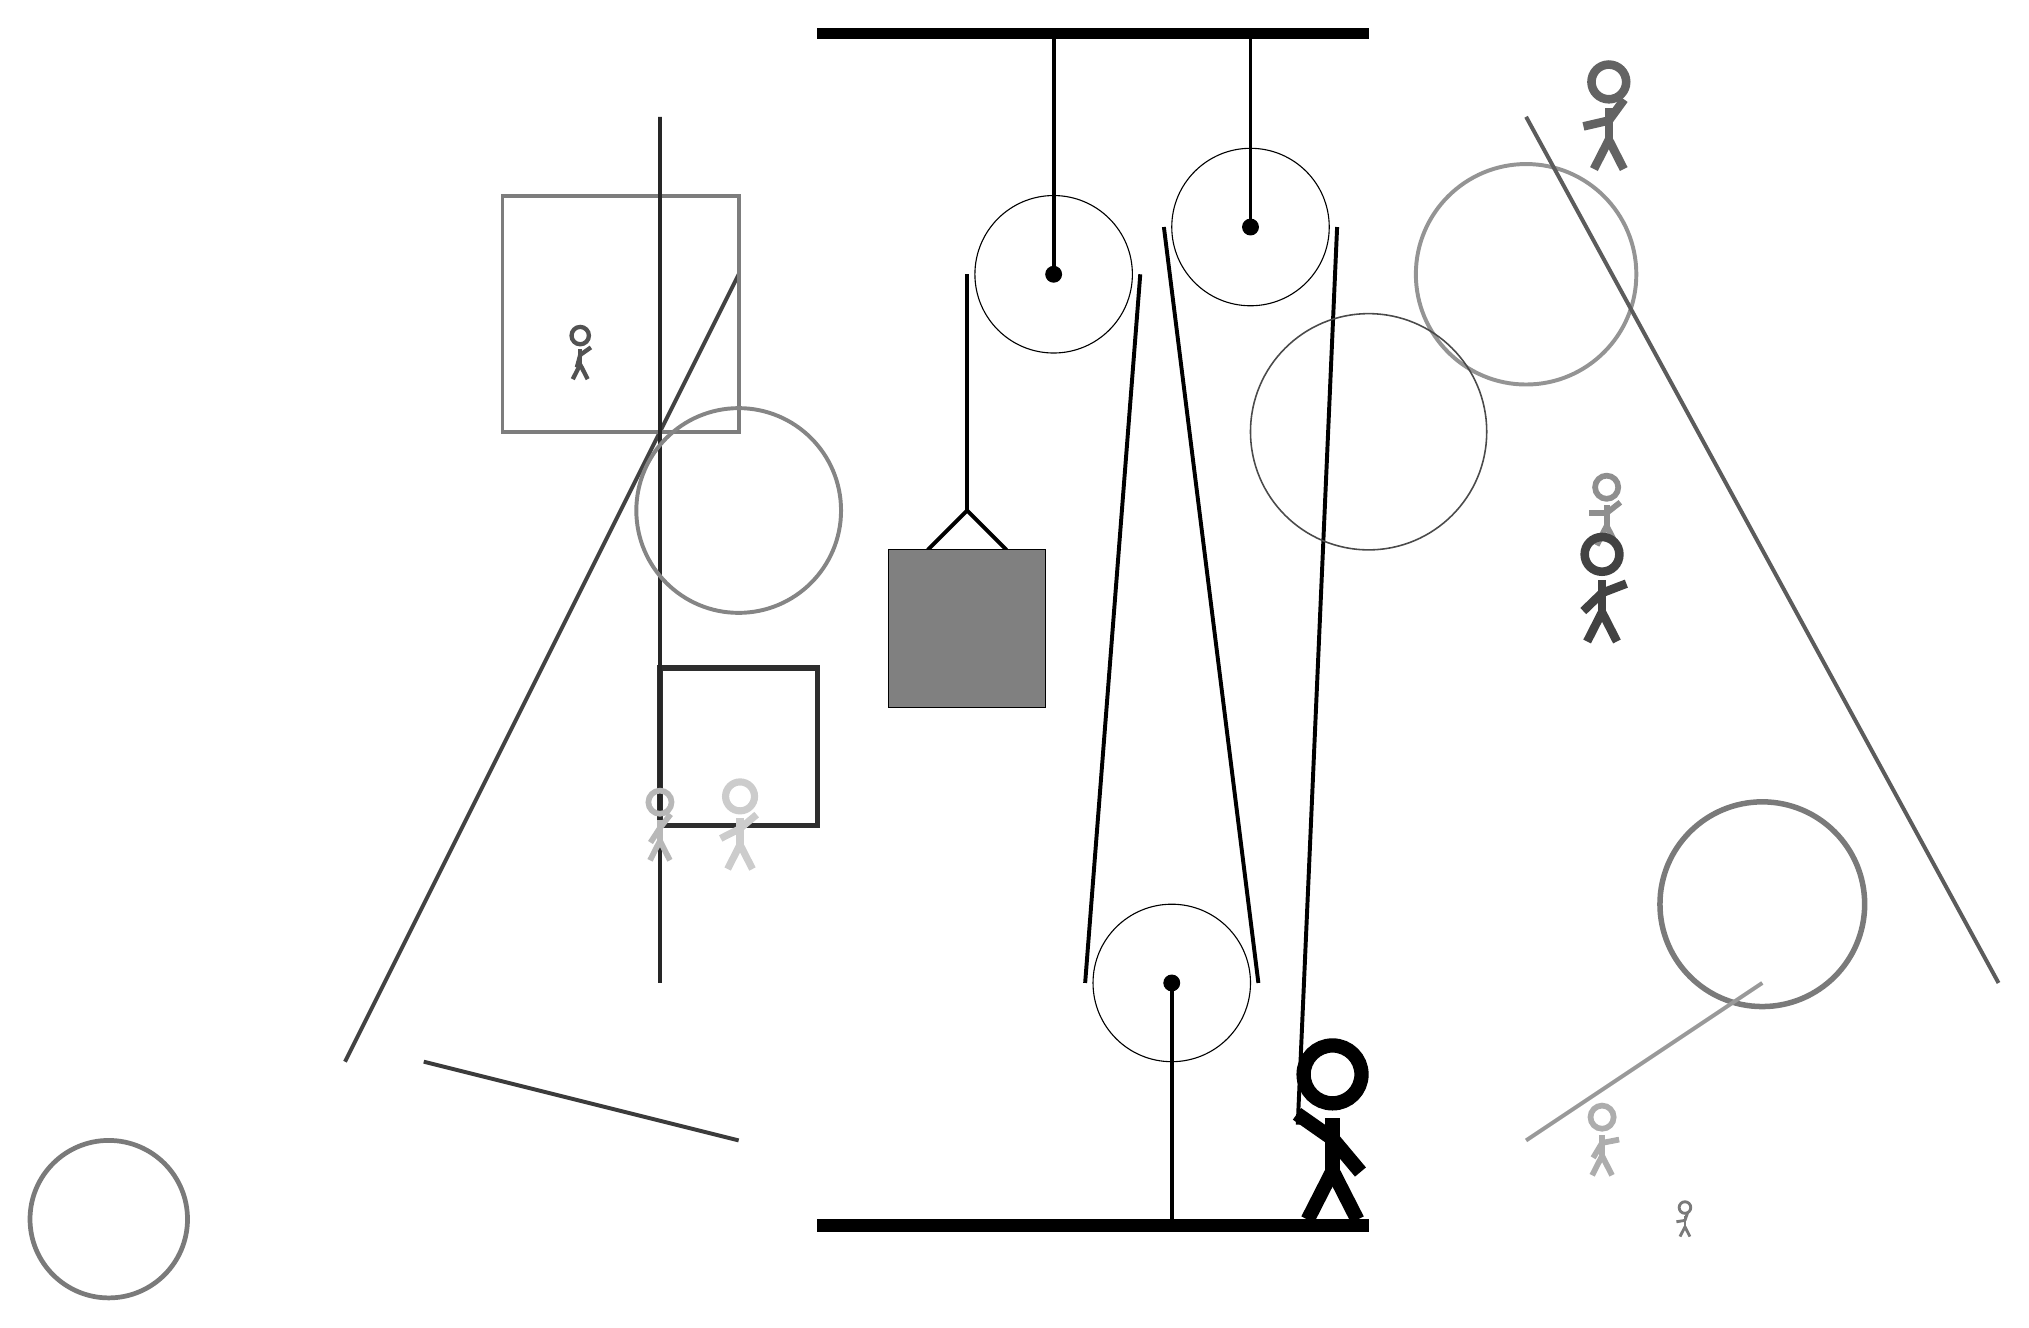
\begin{tikzpicture}
			%%%%% START %%%%%
			
			\draw[fill=black] (-2, 12) rectangle (5, 12.125);
			
			\draw (1, 9) circle (1);
			\draw[fill=black] (1, 9) circle (0.1);
			\draw[line width=0.5mm]  (1, 12) -- (1, 9);
			
			\draw[fill=white](2.5, 0) circle (1);
			\draw[fill=black] (2.5, 0) circle (0.1);
			\draw[line width=0.5mm]  (2.5, -3) -- (2.5, 0);
			
			\draw[fill=white](3.5, 9.6) circle (1);
			\draw[fill=black] (3.5, 9.6) circle (0.1);
			\draw[line width=0.5mm] (3.5, 12) -- (3.5, 9.6);
			
			\draw[line width=0.5mm] (-0.6, 5.5) -- (-0.1, 6.0) -- (0.4, 5.5);
			\draw[fill=black!50] (-1.1, 5.5) rectangle (0.9, 3.5);
			
			\draw[line width=0.5mm] (-0.1, 9) -- (-0.1, 6.0);
			\centerarc[line width=0.5mm](1, 9)(0:180:1.1);
			\draw[line width=0.5mm](2.1, 9) -- (1.4, 0);
			\centerarc[line width=0.5mm](2.5, 0)(180:360:1.1);
			\draw[line width=0.5mm](3.6, 0) -- (2.4, 9.6);
			\centerarc[line width=0.5mm](3.5, 9.6)(0:180:1.1);
			\draw[line width=0.5mm](4.6, 9.6) -- (4.1, -1.8);
			
			\node at (4.5, -1.9) {\Strichmaxerl[10][-35][-50]};
			
			\draw [line width=0.5mm, color=black!42](7, 9) circle (1.4);
			
			\draw[line width=0.7mm, color=black!82] (-2, 2) rectangle (-4, 4);
			\draw[line width=0.5mm, color=black!74](-3, 9) -- (-8, -1);
			\node[line width=0.5mm, color=black!68] at (-5, 8) {\Strichmaxerl[3][75][35]};
			\draw[line width=0.5mm, color=black!64](7, 11) -- (13, 0);
			
			\node[line width=0.4mm, color=black!44] at (8, 6) {\Strichmaxerl[4][0][38]};
			
			\draw [line width=0.2mm, color=black!71](5, 7) circle (1.5);
			\node[line width=0.3mm, color=black!74] at (8, 5) {\Strichmaxerl[6][44][21]};
			\draw [line width=0.7mm, color=black!52](10, 1) circle (1.3);
			
			\draw[line width=0.5mm, color=black!51] (-3, 7) rectangle (-6, 10);
			
			\node[line width=0.4mm, color=black!32] at (8, -2) {\Strichmaxerl[4][59][11]};
			\node[line width=0.4mm, color=black!52] at (9, -3) {\Strichmaxerl[2][9][71]};
			\node[line width=0.6mm, color=black!61] at (8, 11) {\Strichmaxerl[6][13][54]};
			
			\draw[line width=0.6mm, color=black!88] (5, 2) rectangle (5, 2);
			\draw[line width=0.4mm, color=black!85] (-4, 11) rectangle (-4, 0);
			\node[line width=0.2mm, color=black!28] at (-4, 2) {\Strichmaxerl[4][57][52]};
			
			\node[line width=0.3mm, color=black!20] at (-3, 2) {\Strichmaxerl[5][27][40]};
			\draw[line width=0.5mm, color=black!40](7, -2) -- (10, 0);
			\draw [line width=0.6mm, color=black!52](-11, -3) circle (1.0);
			
			\draw [line width=0.5mm, color=black!48](-3, 6) circle (1.3);
			\draw[line width=0.5mm, color=black!77](-7, -1) -- (-3, -2);
			
			
			\draw[fill=black] (-2, -3) rectangle (5, -3.15);
			
			%%%%% END %%%%%
		\end{tikzpicture}
	\end{figure}	
\end{document}